% Copyright 2026 Sreeram Anil
% SPDX-License-Identifier: CC-BY-4.0
\chapter{Bootstrap particle filter (PF-Bootstrap)}
\label{ch:pfbootstrap}

\section*{At a glance}
\begin{tabular}{@{}l>{\raggedright\arraybackslash}p{0.76\textwidth}@{}}
Family & Sequential Monte Carlo (particle / ensemble / Gaussian sum) \\
Header & \texttt{include/estkit/particle/pf\_bootstrap.hpp} \\
Registered name & \texttt{PF-Bootstrap} ($N=500$ particles) \\
State dimension & $n_x = 4$ (cell model) — generic in $n_x, n_u, n_y$ \\
Cost per step & $\mathcal{O}(N(n_x^2 + c_f + c_h))$; \SI{76.4}{\micro\second}/step ($160\times$ EKF), no heap \\
Memory & \SI{46.5}{\kilo\byte} (two $N\times n_x$ state arrays, weights, indices) \\
Primary references & \cite{gordon1993,arulampalam2002,kitagawa1996,doucet2000smc} \\
\end{tabular}

\section{Motivation and aerospace/BMS relevance}
Every filter in this report that carries a covariance matrix answers the filtering
problem by assuming that the posterior $p(\vx_k \mid \vy_{1:k})$ is (approximately) Gaussian and
that the model is (approximately) affine over the support of that Gaussian.  For a lithium-ion
cell both assumptions are comfortable most of the time and uncomfortable exactly when the estimate
matters: near an empty pack the open-circuit-voltage curve $\ocv(\soc)$ has a knee, so a symmetric
SOC uncertainty maps to a strongly skewed voltage uncertainty; after a sensor dropout or a
mis-initialisation the SOC posterior can be genuinely multi-modal, because two different states of
charge with different hysteresis levels can reproduce the same terminal voltage.

The bootstrap filter of Gordon, Salmond and Smith \cite{gordon1993} removes both assumptions.  It
represents the posterior by a weighted cloud of state samples --- \emph{particles} --- propagated
through the true nonlinear dynamics and re-weighted by the true likelihood.  Nothing is
linearised, nothing is assumed Gaussian, and constraints such as $\soc \in [-0.05, 1.05]$ are
enforced by construction because every particle is a physically admissible state.  The price is
computation: the method is three orders of magnitude more expensive per step than an EKF and its
error decays only as $N^{-1/2}$.

In aerospace practice the bootstrap filter is the reference implementation against which cheaper
approximations are validated: it is used offline, on recorded flight data, to establish what the
achievable accuracy of a given sensor suite actually is, and it is used online only where the
posterior is known to be non-Gaussian (terrain-aided navigation, track-before-detect radar,
fault-mode isolation).  For a battery-management unit the same division of labour applies --- an
EKF flies, a particle filter certifies --- and the present chapter quantifies the gap on the eVTOL
mission.  Particle filters have also been proposed directly for cell-level SOC/SOH estimation
\cite{schwunk2013pf}; the results below explain why they rarely displace the sigma-point filters
in that role.

\section{Problem statement and assumptions}
The plant is the generic discrete-time model of \code{core/model.hpp},
\begin{align}
  \vx_k &= f(\vx_{k-1}, \vu_{k-1}) + \vw_{k-1}, & \vw_{k-1} &\sim \N{\bm{0}}{\mQ(\vx,\vu)},
  \label{eq:pfb-dyn} \\
  \vy_k &= h(\vx_k, \vu_k) + \vv_k, & \vv_k &\sim \N{\bm{0}}{\mR(\vx,\vu)},
  \label{eq:pfb-meas}
\end{align}
with state $\vx_k \in \real^{n_x}$, input $\vu_k \in \real^{n_u}$, measurement
$\vy_k \in \real^{n_y}$, and mutually independent white noises $\vw$, $\vv$ that are independent of
the initial state $\vx_0 \sim p(\vx_0)$.  The filter requires only
\begin{enumerate}[label=(A\arabic*),leftmargin=3em]
  \item the ability to \emph{sample} from the transition density
        $p(\vx_k \mid \vx_{k-1}) = \N{f(\vx_{k-1},\vu_{k-1})}{\mQ}$, and
  \item the ability to \emph{evaluate} the likelihood
        $p(\vy_k \mid \vx_k) = \N{h(\vx_k,\vu_k)}{\mR}$ pointwise up to a constant.
\end{enumerate}
Gaussianity of $\vw$ and $\vv$ is used only in the implementation; neither the derivation nor the
code structure needs it.  What is \emph{not} assumed: linearity of $f$ or $h$, unimodality of
$p(\vx_0)$, or existence of the Jacobians $\mF$, $\mH$.

The quantity to be estimated is the minimum-mean-square-error state,
$\xhat_k = \E{\vx_k \mid \vy_{1:k}}$, together with its covariance
$\mP_k = \Var{\vx_k \mid \vy_{1:k}}$, which the benchmark reports as
\code{soc\_std} $=\sqrt{(\mP_k)_{\soc\soc}}$.

\section{Derivation}

\subsection{The exact recursion}
Bayes' rule and the Markov property give the two-step recursion that every filter approximates
\cite[\S{}II]{arulampalam2002}:
\begin{align}
  p(\vx_k \mid \vy_{1:k-1}) &= \int p(\vx_k \mid \vx_{k-1})\, p(\vx_{k-1}\mid\vy_{1:k-1})\, d\vx_{k-1},
  \label{eq:pfb-chapman}\\
  p(\vx_k \mid \vy_{1:k}) &= \frac{p(\vy_k\mid\vx_k)\, p(\vx_k\mid\vy_{1:k-1})}
                                  {\int p(\vy_k\mid\vx_k)\, p(\vx_k\mid\vy_{1:k-1})\, d\vx_k}.
  \label{eq:pfb-bayes}
\end{align}
Outside the linear-Gaussian case the integrals have no closed form.  The Kalman family evaluates
them by moment matching; sequential Monte Carlo evaluates them by importance sampling.

\subsection{Importance sampling and the weight recursion}
Let $\vx_{0:k}$ denote a state trajectory and let $q(\vx_{0:k}\mid\vy_{1:k})$ be an
\emph{importance density} that is easy to sample from and whose support contains that of the
posterior.  For any test function $g$,
\begin{equation}
  \E{g(\vx_{0:k}) \mid \vy_{1:k}}
  = \frac{\displaystyle\int g(\vx_{0:k})\,
          \frac{p(\vx_{0:k}\mid\vy_{1:k})}{q(\vx_{0:k}\mid\vy_{1:k})}\, q(\vx_{0:k}\mid\vy_{1:k})\, d\vx_{0:k}}
         {\displaystyle\int \frac{p(\vx_{0:k}\mid\vy_{1:k})}{q(\vx_{0:k}\mid\vy_{1:k})}\, q(\vx_{0:k}\mid\vy_{1:k})\, d\vx_{0:k}},
  \label{eq:pfb-is}
\end{equation}
so drawing $\vx_{0:k}^i \sim q$, $i = 1,\dots,N$, and setting the \emph{unnormalised importance
weight} $\tilde w_k^i \propto p(\vx_{0:k}^i\mid\vy_{1:k}) / q(\vx_{0:k}^i\mid\vy_{1:k})$ yields the
self-normalised estimator
\begin{equation}
  \E{g \mid \vy_{1:k}} \approx \sum_{i=1}^{N} w_k^i\, g(\vx_{0:k}^i),
  \qquad w_k^i = \tilde w_k^i \Big/ \sum_{j=1}^{N} \tilde w_k^j .
  \label{eq:pfb-selfnorm}
\end{equation}
Choosing an importance density that factorises,
$q(\vx_{0:k}\mid\vy_{1:k}) = q(\vx_k \mid \vx_{0:k-1},\vy_{1:k})\, q(\vx_{0:k-1}\mid\vy_{1:k-1})$,
makes the weights recursive.  Substituting the factorisation
$p(\vx_{0:k}\mid\vy_{1:k}) \propto p(\vy_k\mid\vx_k) p(\vx_k\mid\vx_{k-1}) p(\vx_{0:k-1}\mid\vy_{1:k-1})$
gives the \emph{sequential importance sampling} (SIS) recursion
\begin{equation}
  \boxed{\;
  \tilde w_k^i = \tilde w_{k-1}^i \,
    \frac{p(\vy_k \mid \vx_k^i)\; p(\vx_k^i \mid \vx_{k-1}^i)}
         {q(\vx_k^i \mid \vx_{0:k-1}^i, \vy_{1:k})} \; }
  \label{eq:pfb-sis}
\end{equation}
\cite[eq.~(47)]{arulampalam2002}.  Every particle filter in this family differs only in the choice
of $q$.  The \emph{bootstrap} choice is the transition prior,
\begin{equation}
  q(\vx_k \mid \vx_{0:k-1}^i, \vy_{1:k}) = p(\vx_k \mid \vx_{k-1}^i),
  \label{eq:pfb-prior-proposal}
\end{equation}
which reduces \eqref{eq:pfb-sis} to the likelihood-only update of Gordon et al.\
\cite[eq.~(12)]{gordon1993}:
\begin{equation}
  \tilde w_k^i = \tilde w_{k-1}^i \; p(\vy_k \mid \vx_k^i),
  \qquad
  \vx_k^i \sim \N{f(\vx_{k-1}^i,\vu_{k-1})}{\mQ}.
  \label{eq:pfb-boot}
\end{equation}
The empirical filtering distribution is then
$\hat p(\vx_k\mid\vy_{1:k}) = \sum_i w_k^i \delta(\vx_k - \vx_k^i)$, and the reported estimates are
its first two moments
\begin{equation}
  \xhat_k = \sum_{i} w_k^i \vx_k^i, \qquad
  \mP_k   = \sum_{i} w_k^i (\vx_k^i - \xhat_k)(\vx_k^i - \xhat_k)^\T .
  \label{eq:pfb-moments}
\end{equation}
Under mild conditions the estimator \eqref{eq:pfb-selfnorm} is consistent and asymptotically
normal with a variance of order $N^{-1}$ uniformly in $k$, provided the dynamics mix; see Crisan
and Doucet \cite{crisan2002convergence} for the precise statements a practitioner should know
(in particular, the uniform-in-time result requires the filter to forget its initial condition,
which is exactly what the near-integrator SOC dynamics do \emph{not} do).

\subsection{Degeneracy and the effective sample size}
The variance of the weights in \eqref{eq:pfb-sis} can only grow with $k$ \cite[Prop.~1]{doucet2000smc}:
after enough steps a single particle carries essentially all of the mass and the other $N-1$
trajectories contribute nothing but cost.  The standard diagnostic is the \emph{effective sample
size} of Kong, Liu and Wong \cite{kong1994},
\begin{equation}
  N_{\mathrm{eff}} = \frac{1}{\sum_{i=1}^N (w_k^i)^2} \in [1, N],
  \label{eq:pfb-ess}
\end{equation}
which equals $N$ for uniform weights and $1$ for a degenerate cloud; it estimates the number of
samples that an i.i.d.\ sampler from the posterior would need to match the variance of the weighted
estimator.  Resampling is triggered when $N_{\mathrm{eff}} < \beta N$; the implementation uses the
usual $\beta = 1/2$ \cite{liuchen1998,arulampalam2002}.

\subsection{Resampling}
Resampling replaces the weighted cloud $\{\vx^i, w^i\}$ by an unweighted cloud
$\{\vx^{a(j)}, 1/N\}$ in which particle $i$ appears $n^i$ times, with the unbiasedness requirement
$\E{n^i} = N w^i$.  Four schemes are in common use (multinomial, stratified, systematic,
residual); Douc, Cappé and Moulines \cite{douc2005resampling} and Hol, Schön and Gustafsson
\cite{hol2006resampling} compare their variance and cost.  \emph{Systematic} resampling
\cite[\S3]{kitagawa1996} is used here: it draws a \emph{single} uniform $u_0\sim\mathcal{U}[0,1)$
and places a deterministic comb on the cumulative weight axis,
\begin{equation}
  u_j = \frac{j + u_0}{N}, \quad j = 0,\dots,N-1,
  \qquad
  a(j) = \min\Big\{ i : \textstyle\sum_{m \le i} w^m \ge u_j \Big\},
  \label{eq:pfb-systematic}
\end{equation}
so that $n^i \in \{\lfloor N w^i\rfloor, \lceil N w^i \rceil\}$ deterministically.  It needs one
random number, one pass, no sorting, and has the lowest Monte-Carlo variance of the four in
practice; these properties also make it the only scheme worth implementing on a microcontroller.

\begin{algorithm}[H]
\caption{Systematic resampling (Kitagawa 1996)}
\begin{algorithmic}[1]
\Require normalised weights $w^1,\dots,w^N$, one uniform $u_0 \sim \mathcal{U}[0,1)$
\State $u \gets u_0/N$, \; $c \gets w^1$, \; $i \gets 1$
\For{$j = 1$ \textbf{to} $N$}
  \While{$u > c$ \textbf{and} $i < N$} \State $i \gets i+1$; \; $c \gets c + w^i$ \EndWhile
  \State $a(j) \gets i$; \quad $u \gets u + 1/N$
\EndFor
\Ensure parent indices $a(1),\dots,a(N)$, each new weight $1/N$
\end{algorithmic}
\end{algorithm}

\subsection{Roughening: why resampling alone is not enough}
Resampling fights weight degeneracy but creates \emph{sample impoverishment}: children are exact
copies of their parents, so the number of distinct particles can only decrease, and for a state
with little process noise the cloud collapses onto a single value that subsequent measurements can
no longer move.  Gordon et al.\ \cite[\S4.2]{gordon1993} therefore add an independent jitter after
every resampling,
\begin{equation}
  \vx^i \leftarrow \vx^i + \bm{J}^i, \qquad
  \bm{J}^i \sim \N{\bm{0}}{\diag(\sigma_1^2,\dots,\sigma_{n_x}^2)}, \qquad
  \sigma_k = K\, E_k\, N^{-1/n_x},
  \label{eq:pfb-roughen}
\end{equation}
where $E_k$ is the spread (maximum minus minimum) of the cloud in coordinate $k$ and $K \approx
0.2$.  The factor $N^{-1/n_x}$ is the mean spacing of $N$ points in an $n_x$-dimensional unit
hypercube, so the jitter exactly fills the gaps that resampling opens, and its effect vanishes as
$N\to\infty$.  Equivalently, \eqref{eq:pfb-roughen} declares an \emph{artificial dynamic noise}:
the transition density is taken to be
$\N{f(\vx_{k-1})}{\mQ + \diag(\sigma^2)}$ rather than $\N{f(\vx_{k-1})}{\mQ}$, so the weight
recursion \eqref{eq:pfb-boot} remains exact for the perturbed model.

Rule \eqref{eq:pfb-roughen} is a positive feedback --- the jitter is proportional to the spread,
which the jitter increases --- and Section~\ref{sec:pfb-battery} shows that on the cell model it
diverges.  The implementation therefore clips it,
\begin{equation}
  \sigma_k = \operatorname{clip}\!\Big( K\,E_k\,N^{-1/n_x};\;
      \underbrace{\varphi_{\min}\sqrt{(\mP_0)_{kk}}}_{\text{floor}},\;
      \underbrace{\varphi_{\max}\sqrt{(\mP_0)_{kk}}}_{\text{cap}} \Big),
  \label{eq:pfb-roughen-clip}
\end{equation}
with $\operatorname{clip}(x;a,b)=\min(\max(x,a),b)$ and both bounds expressed as fractions of the \emph{prior}
standard deviation handed to \code{init()}, which keeps the rule model-independent.  The floor
prevents terminal impoverishment ($E_k \to 0 \Rightarrow \sigma_k \to 0$); the cap removes the
feedback.  Defaults: $K = 0.2$, $\varphi_{\min} = 0.005$, $\varphi_{\max}=0.02$.

\section{Algorithm}
\begin{algorithm}[H]
\caption{PF-Bootstrap --- one sampling period}
\begin{algorithmic}[1]
\Require particles $\{\vx_{k-1}^i\}$ and log-weights $\{\ell_{k-1}^i\}$, inputs $\vu_{k-1},\vu_k$, measurement $\vy_k$
\State \textbf{Time update (\code{predict}).}  $\mL_Q \gets \operatorname{chol}(\mQ(\xhat_{k-1},\vu_{k-1}))$
\For{$i = 1$ \textbf{to} $N$}
  \State $\vx_k^i \gets f(\vx_{k-1}^i, \vu_{k-1}) + \mL_Q \,\bm{\xi}^i$, \quad $\bm{\xi}^i \sim \N{\bm{0}}{\mI}$
  \State $\vx_k^i \gets \operatorname{constrain}(\vx_k^i)$
\EndFor
\State \textbf{Prior predictive (\code{predict\_measurement}).} $\yhat_k \gets \sum_i w_{k-1}^i\, h(\vx_k^i, \vu_k)$
\State \textbf{Measurement update (\code{update}).} $\mL_R \gets \operatorname{chol}(\mR)$; \; $c_0 \gets -\sum_m \log (\mL_R)_{mm} - \tfrac{n_y}{2}\log 2\pi$
\For{$i = 1$ \textbf{to} $N$}
  \State $\veps^i \gets \vy_k - h(\vx_k^i,\vu_k)$; \quad
         $\ell_k^i \gets \ell_{k-1}^i + c_0 - \tfrac12 \norm{\mL_R^{-1}\veps^i}^2$
\EndFor
\State $w_k^i \gets \exp(\ell_k^i - \max_j \ell_k^j) \big/ \sum_m \exp(\ell_k^m - \max_j \ell_k^j)$;\quad $\ell_k^i \gets \log w_k^i$
\State $N_{\mathrm{eff}} \gets 1/\sum_i (w_k^i)^2$
\If{$N_{\mathrm{eff}} < \beta N$}
  \State systematic resampling $\to$ parents $a(j)$; \; $\vx_k^j \gets \vx_k^{a(j)}$, \; $w_k^j \gets 1/N$
  \State roughening \eqref{eq:pfb-roughen-clip}; \; $\vx_k^j \gets \operatorname{constrain}(\vx_k^j)$
\EndIf
\State $\xhat_k \gets \sum_i w_k^i \vx_k^i$; \quad
       $\mP_k \gets \sum_i w_k^i (\vx_k^i-\xhat_k)(\vx_k^i-\xhat_k)^\T$
\Ensure $\xhat_k$, $\mP_k$, $\{\vx_k^i, w_k^i\}$
\end{algorithmic}
\end{algorithm}

\section{Application to the battery model}
\label{sec:pfb-battery}
For the cell model $\vx = [\soc, v_1, v_2, h]^\T$, $\vu = [i, T]^\T$, $y = v$ of
Chapter~\ref{ch:ecm} every particle is an independent copy of the ESC model: the SOC integrator,
the two RC branches and the hysteresis state are propagated by $f$ exactly as the EKF propagates
its mean, and the likelihood is the scalar Gaussian
\begin{equation}
  p(v_k \mid \vx_k^i) = \N{\ocv(\soc^i,T) + M h^i - v_1^i - v_2^i - R_0(T) i_k}{\sigma_v^2 + (R_0 \sigma_i)^2}.
  \label{eq:pfb-celllik}
\end{equation}
Three model-specific observations drive every design choice in the header.

\paragraph{The likelihood is far sharper than the process noise.}
With $\sigma_v = \SI{2}{\milli\volt}$ and $\partial \ocv/\partial \soc \approx
\SI{0.7}{\volt}$ per unit SOC, one voltage sample resolves SOC to
$\sigma_v / |\partial\ocv/\partial\soc| \approx 0.003$, whereas the per-step SOC process noise is
$q_{\soc}^{1/2} = 10^{-5}$.  The transition prior \eqref{eq:pfb-prior-proposal} therefore proposes
particles into a region $300$ times narrower than the likelihood can discriminate; the weights
concentrate immediately, $N_{\mathrm{eff}}$ falls below $N/2$ at essentially every step, and the
filter resamples at \SI{10}{\hertz}.  This is the regime in which the auxiliary
(Chapter~\ref{ch:pfauxiliary}) and unscented (Chapter~\ref{ch:upf}) proposals are supposed to help.

\paragraph{Roughening is mandatory, and the textbook rule diverges.}
Because $q_{\soc}$ is negligible, resampling without jitter freezes the SOC spread within a few
steps and the filter degenerates into open-loop Coulomb counting from whatever SOC it happened to
collapse onto.  Applying \eqref{eq:pfb-roughen} with Gordon's $K=0.2$ and no cap, however, makes
the filter diverge: measured on the nominal eVTOL mission (development run, seed 1), SOC
$\mathrm{RMSE}_{\mathrm{ss}} = \SI{49.5}{\percent}$ with $v_2$ drifting to \SI{0.6}{\volt}.  The mechanism is
worth stating because it applies to every jitter-based scheme (and, in the covariance-inflation
form, to the ensemble filters of Chapters~\ref{ch:enkf}--\ref{ch:etkf}): within one \SI{0.1}{\second}
step the terminal voltage cannot distinguish an SOC change from an equal and opposite change of
$v_1 + v_2$, so the direction $\partial v/\partial(\soc, v_2)$ is nearly unobservable; the jitter
inflates the cloud along that direction faster than the measurement contracts it, and the excess
spread feeds back into a larger jitter.  Capping $\sigma_k$ at $2\,\%$ of the prior standard
deviation removes the feedback and restores $\mathrm{RMSE}_{\mathrm{ss}} = \SI{0.13}{\percent}$ on
the same run --- a factor of \num{380}.  The floor at $0.5\,\%$ of the prior standard deviation
($\sigma_{\soc} = 5\times10^{-4}$ per step here) is what lets the cloud walk \SI{35}{\percent} of
SOC during the \code{init\_error} scenario.

\paragraph{$\mQ$ and $\mR$ are evaluated once per step at the cloud mean.}
For the ECM both depend on the state only through the hysteresis row of $\mB$, whose contribution
is three orders of magnitude below the diagonal floors; evaluating them per particle would triple
the cost of the time update for no measurable accuracy gain.  \code{Options} keeps
\code{q\_scale}/\code{r\_scale} for tuning, and a model whose $\mQ$ genuinely depends on $\vx$
would need the per-particle factorisation reinstated (four lines).

\section{Implementation notes}
\emph{Storage.}  Two $N \times n_x$ arrays of \code{Real} (particles and the resampling buffer),
two $N$-vectors of weights and log-weights, and an $N$-vector of parent indices:
$\SI{46.5}{\kilo\byte}$ at $N=500$ in double precision, all as members so that nothing touches the
stack or the heap.  Chapter~\ref{ch:pffast} removes the resampling buffer.

\emph{Numerics.}  Weights are carried as log-weights and normalised with the max-shift
$w^i = e^{\ell^i - \ell_{\max}} / \sum_j e^{\ell^j-\ell_{\max}}$, without which the recursion
underflows: the log-likelihood spread across the cloud routinely exceeds $-800$ (the double
underflow limit) and $-90$ (the float limit) during the initial transient.  After normalisation the
log-weights are recentred, $\ell^i \leftarrow \ell^i - \log\sum_j e^{\ell^j}$, so they stay
$\mathcal{O}(1)$ for the whole mission.  The likelihood is evaluated through the inverse Cholesky
factor of $\mR$ computed once per step, so the per-particle work contains no transcendental
function beyond the single $\exp$ of the normalisation.  $\mP_k$ is accumulated in the upper
triangle and mirrored, which keeps it exactly symmetric.

\emph{Float32.}  The whole family compiles and runs with \code{-DESTKIT\_FLOAT=ON}, and the
single-precision build costs essentially nothing: on \code{nominal} the bootstrap filter gives
$\mathrm{RMSE}_{\mathrm{ss}} = \SI{0.18}{\percent}$ in double and \SI{0.17}{\percent} in float
(Table~\ref{tab:float}), the difference being Monte-Carlo noise rather than round-off.  The reason is
the max-shifted normalisation: the only quantity with a large dynamic range never leaves the log
domain, and the cumulative-weight sum of \eqref{eq:pfb-systematic} is a sum of $N$ numbers of
comparable size.

\emph{Cost.}  Per step: $N$ evaluations of $f$, $2N$ of $h$ (one for the prior predictive, one for
the weight), $N n_x$ Gaussian draws, one $n_x\times n_x$ and one $n_y \times n_y$ Cholesky, and
$\mathcal{O}(N n_x^2)$ for the moments.  Measured: \SI{76.4}{\micro\second}/step on the benchmark
machine, i.e.\ $160\times$ the EKF (\SI{477}{\nano\second}).  The runtime table's projection to a
Cortex-M7 class processor ($\kappa=30$, Chapter~\ref{ch:metrics}) is \SI{2.3}{\milli\second}/step,
so $N=500$ at \SI{10}{\hertz} is feasible but consumes about $2.3\,\%$ of the CPU per cell ---
untenable for a 100-cell pack, which is the practical argument for Chapters~\ref{ch:pffast} and \ref{ch:rbpf}.

\emph{Reproducibility.}  The RNG is the deterministic \code{xoshiro256**} stream of
\code{core/rng.hpp}, seeded from \code{EstimatorConfig::seed} through \code{seed()} in the
registration lambda, so a given seed reproduces the run bit-for-bit on any platform.

\section{Benchmark results}
% Copyright 2026 Sreeram Anil
% SPDX-License-Identifier: CC-BY-4.0
\begin{table}[H]\centering\footnotesize\setlength{\tabcolsep}{4pt}
\caption{PF-Bootstrap: cell-level benchmark on the eVTOL mission (mean over seeds; RMSE and max error in \% SOC; $t_\mathrm{conv}$: first time the error stays below 2\,\% for 60\,s, -- = never; EKF reference: steady-state RMSE of the plain EKF on the same data).}\label{tab:cell_PFBootstrap}
\begin{tabular}{llrrrrrcrr}\toprule
plant & scenario & RMSE & RMSE$_\mathrm{ss}$ & max & $t_\mathrm{conv}$ [s] & RMSE$_v$ [mV] & div. & EKF ref. & ns/step \\ \midrule
ECM & nominal & 0.17 & 0.16 & 0.75 & 0 & 0.84 & no & 0.05 & 76444 \\
ECM & init\_error & 0.53 & 0.13 & 5.01 & 73 & 2.21 & no & 0.05 & 76795 \\
ECM & current\_bias & 0.87 & 0.87 & 2.07 & 0 & 0.87 & no & 0.61 & 76600 \\
ECM & noise\_step & 0.43 & 0.51 & 1.77 & 0 & 2.94 & no & 0.12 & 89727 \\
ECM & outliers & 0.49 & 0.36 & 1.86 & 0 & 1.56 & no & 0.21 & 78744 \\
ECM & cold & 0.39 & 0.33 & 2.32 & 0 & 1.94 & no & 0.16 & 77053 \\
ECM & hot & 0.12 & 0.08 & 0.71 & 0 & 0.61 & no & 0.03 & 76493 \\
ECM & aged\_cell & 3.27 & 2.54 & 13.94 & 0 & 4.95 & no & 1.52 & 79624 \\
ECM & param\_mismatch & 2.09 & 1.72 & 9.18 & 0 & 3.41 & no & 1.36 & 78697 \\
ECM & sensor\_dropout & 0.29 & 0.13 & 3.32 & 0 & 1.43 & no & 0.46 & 76574 \\
ECM & preisach & 1.52 & 1.08 & 4.56 & 221 & 0.88 & no & 0.20 & 77186 \\
ECM & combined & 3.27 & 2.76 & 15.21 & 277 & 6.43 & no & 12.44 & 79674 \\
\midrule
SPM & nominal & 1.00 & 0.73 & 3.20 & 0 & 1.07 & no & 3.73 & 74498 \\
SPM & init\_error & 1.33 & 0.93 & 5.01 & 132 & 2.20 & no & 3.81 & 74489 \\
SPM & current\_bias & 1.18 & 1.10 & 3.87 & 121 & 1.15 & no & 5.69 & 74834 \\
SPM & noise\_step & 1.22 & 1.11 & 3.20 & 0 & 3.05 & no & 3.30 & 87148 \\
SPM & outliers & 1.28 & 0.96 & 4.50 & 0 & 1.77 & no & 1.99 & 76148 \\
SPM & cold & 4.15 & 4.39 & 14.02 & 988 & 7.32 & no & 7.35 & 75159 \\
SPM & hot & 0.96 & 0.97 & 2.79 & 0 & 0.75 & no & 2.16 & 74422 \\
SPM & param\_mismatch & 2.90 & 1.67 & 8.36 & 781 & 2.16 & no & 3.13 & 75088 \\
SPM & sensor\_dropout & 1.08 & 0.73 & 6.90 & 0 & 2.01 & no & 5.31 & 74452 \\
\bottomrule\end{tabular}\end{table}

\begin{figure}[H]\centering
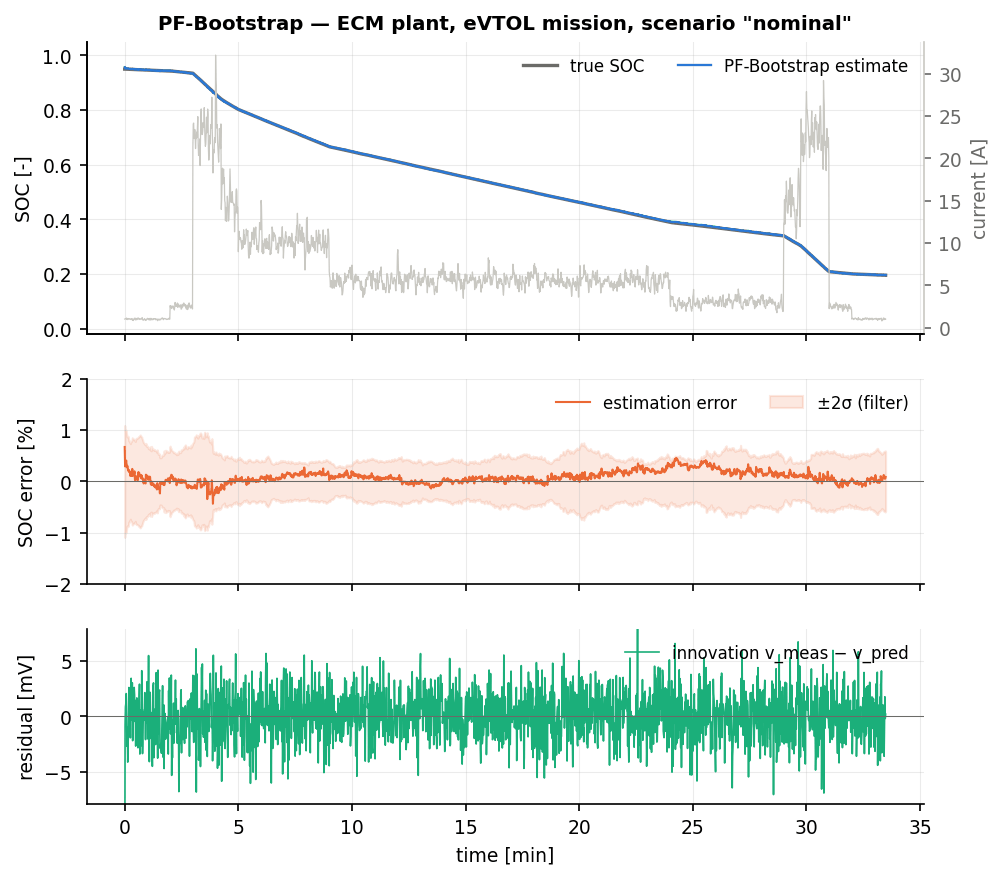
\includegraphics[width=\textwidth]{figures/cell_PFBootstrap_nominal.png}
\caption{PF-Bootstrap on the nominal eVTOL mission: true and estimated SOC (top), estimation error
with the $\pm 2\sigma$ band from the weighted particle covariance (middle), voltage residual (bottom).}
\end{figure}
\begin{figure}[H]\centering
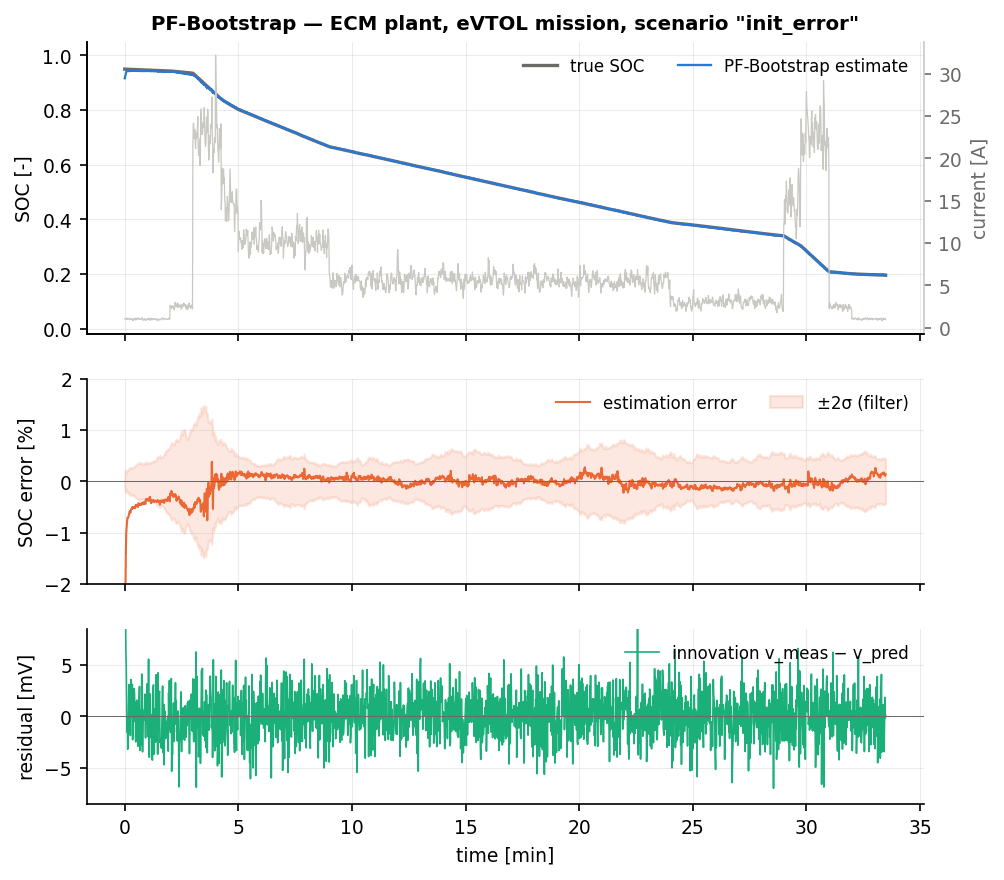
\includegraphics[width=\textwidth]{figures/cell_PFBootstrap_init_error.png}
\caption{PF-Bootstrap with a \SI{35}{\percent} initial SOC error.  The cloud walks to the truth under
the roughening floor; the residual error after the first few seconds is indistinguishable from the
nominal case, but the \SI{2}{\percent} convergence criterion is only met after \SI{73}{\second}
because the slowest of the three seeds spends that long inside the RC transient.}
\end{figure}
\begin{figure}[H]\centering
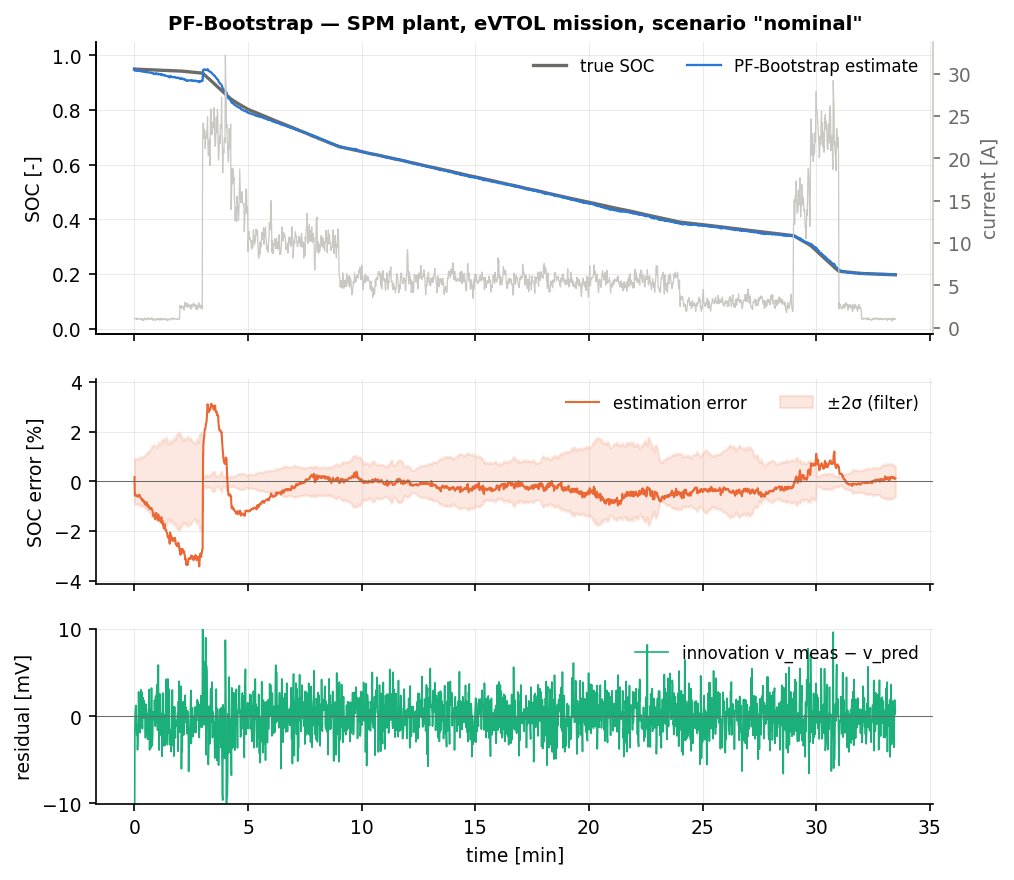
\includegraphics[width=\textwidth]{figures/cellspm_PFBootstrap_nominal.png}
\caption{PF-Bootstrap on the electrochemical (SPM) plant, nominal mission: the estimator's 2-RC ECM
carries a structured \SI{4}{\milli\volt} residual against the true single-particle model, and the
particle cloud absorbs it as spread instead of as SOC bias.}
\end{figure}

\paragraph{ECM plant.}  On \code{nominal} the filter reaches $\mathrm{RMSE} = \SI{0.17}{\percent}$,
$\mathrm{RMSE}_{\mathrm{ss}} = \SI{0.16}{\percent}$ and a maximum error of \SI{0.75}{\percent},
converging immediately, with a voltage-residual RMSE of \SI{0.84}{\milli\volt}.  That is a factor
of three \emph{worse} than the EKF ($\mathrm{RMSE}_{\mathrm{ss}} = \SI{0.05}{\percent}$) at
$160\times$ the cost --- the honest and expected outcome, because the nominal ECM posterior really
is Gaussian, the EKF is then statistically efficient, and the particle filter pays an
$\mathcal{O}(N^{-1/2})$ Monte-Carlo penalty plus the bias of the roughening floor.

Where the cloud earns its keep is in the scenarios that break the Gaussian assumption.  With a
\SI{35}{\percent} initial SOC error the steady-state error is \SI{0.13}{\percent} --- better than
its own nominal value, and equal to the EKF's \SI{0.05}{\percent} to within the Monte-Carlo noise
of three seeds --- with a peak of \SI{5.0}{\percent}: the likelihood simply re-weights the tail of
the prior cloud, and no linearisation of $\ocv$ over a \SI{35}{\percent}-wide SOC interval is ever
required.  In \code{sensor\_dropout} (\SI{15}{\second} of stuck voltage) it is one of the best
methods of the family, $\mathrm{RMSE}_{\mathrm{ss}} = \SI{0.13}{\percent}$ against
\SI{0.46}{\percent} for the EKF and \SI{0.86}{\percent} for the UKF --- a frozen measurement
produces a frozen likelihood that merely stops sharpening the cloud, whereas a Kalman filter keeps
applying a gain to a stale innovation.  In \code{combined} the EKF fails outright
($\mathrm{RMSE}_{\mathrm{ss}} = \SI{12.44}{\percent}$, never converging); the bootstrap filter
stays at \SI{2.76}{\percent}.

The weaknesses are equally systematic.  \code{aged\_cell} (\SI{15}{\percent} capacity loss) gives
\SI{2.54}{\percent} against \SI{1.52}{\percent} for the EKF, and \code{param\_mismatch}
\SI{1.72}{\percent} against \SI{1.36}{\percent}: a particle filter cannot out-estimate a wrong
model, and the roughening jitter --- the only thing keeping the cloud alive --- adds variance
without addressing bias.  \code{noise\_step} (\SI{0.51}{\percent} against \SI{0.12}{\percent} for
the EKF) is the scenario where the fixed $\mR$ hurts most visibly: the filter keeps weighting with
$\sigma_v = \SI{2}{\milli\volt}$ after the sensor noise jumps to \SI{20}{\milli\volt}, so the
weights become far too aggressive.  An adaptive $\mR$ of the Sage--Husa type \cite{sagehusa1969}
would fix that and is orthogonal to the sampling scheme.  The clearest regression against the
development runs is \code{preisach}: with the corrected hysteresis sign convention the unmodelled
Preisach loop acts as a slowly varying \emph{bias} on the terminal voltage, and the bootstrap
filter converts that bias into an SOC offset of \SI{1.08}{\percent} where the EKF, whose single
hysteresis state absorbs part of it linearly, stays at \SI{0.20}{\percent}.  Sampling fidelity is
of no help against an unmodelled mechanism.

\paragraph{SPM plant.}  On the electrochemical plant the ranking inverts, and decisively.  The
estimators run a 2-RC ECM fitted to the single-particle model, which leaves a structured
\SI{4}{\milli\volt} residual (Butler--Volmer kinetics, slow solid diffusion, $\tau_2 =
\SI{556}{\second}$) --- a model error that is neither white nor small.  The bootstrap filter gives
$\mathrm{RMSE}_{\mathrm{ss}} = \SI{0.73}{\percent}$ on \code{nominal} against \SI{3.73}{\percent}
for the EKF: a factor of \num{5.1}.  The advantage holds across the SPM scenario set ---
\code{current\_bias} \SI{1.10}{\percent} against \SI{5.69}{\percent}, \code{sensor\_dropout}
\SI{0.73}{\percent} against \SI{5.31}{\percent}, \code{param\_mismatch} \SI{1.67}{\percent} against
\SI{3.13}{\percent}, \code{cold} \SI{4.39}{\percent} against \SI{7.35}{\percent} --- and no SPM
scenario diverges.

The mechanism is worth stating precisely, because it is the strongest argument in this chapter for
sampling.  A structured voltage residual has to be absorbed by \emph{something}.  In a Kalman
filter the absorber is chosen by the linearised gain: over one sample interval the residual is
almost equally explainable by a change in $\soc$ or by an equal and opposite change in $v_1+v_2$,
and the gain --- computed from a covariance whose $\soc$ block has long since collapsed --- puts it
largely into $\soc$, which then stays wrong because the model keeps re-creating the residual.  The
particle cloud is not tied to that linearised $(\soc, v_2)$ ambiguity: particles with different
SOC \emph{and} different RC states coexist, the likelihood keeps whichever combination reproduces
the measured voltage, and the roughening jitter continuously re-supplies the diversity that lets
the slow RC state, rather than the SOC, take up the persistent part of the residual.  The result is
that the model error surfaces as voltage-residual RMSE (\SI{1.07}{\milli\volt} on SPM
\code{nominal}, up from \SI{0.84}{\milli\volt} on the ECM) instead of as an SOC bias.  The price
was visible in the ECM rows: the same jitter costs a factor of three in nominal accuracy when the
model happens to be exact.

\section{Summary}
The bootstrap filter is the reference implementation of Bayesian filtering: it makes no Gaussian or
linearity assumption, needs no Jacobians, keeps every particle physically admissible, and converges
to the exact posterior as $N\to\infty$.  On the \emph{matched} cell model it costs $160\times$ an
EKF and is three times less accurate in nominal conditions, so it is not the filter to ship in a
BMS when the model is trusted.  On the \emph{mismatched} electrochemical plant --- the realistic
case --- it is five times \emph{more} accurate than the EKF (\SI{0.73}{\percent} against
\SI{3.73}{\percent}), because a cloud can distribute a structured residual over SOC and the RC
states while a linearised gain cannot.  It is also immune to the EKF's \code{combined}-scenario
failure and one of the best methods on \code{sensor\_dropout}.  Its two practical hazards are
sample impoverishment (cured by a roughening floor) and the positive feedback of the classical
roughening rule in weakly observable directions (cured by a cap); both are quantified above and
both are one line of \code{Options}.
